El contenido de este cap\'{\i}tulo es f\'acil de describir: un programa consiste
esencialmente en bloques \lstinline|for|, que repiten un n\'umero de veces un
grupo de instrucciones, y bloques \lstinline|if|, que bifurcan la ejecuci\'on
del c\'odigo seg\'un se cumplan o no determinadas condiciones booleanas: si se
cumple una condici\'on ejecutan un bloque de instrucciones y si no se cumple
otro distinto. 

Se describe la sintaxis de ambos tipos de bloque y se muestra mediante ejemplos
sencillos su uso, junto con otros m\'etodos como la recursi\'on y los bloques
\lstinline|while|. 

Como se indic\'o en el pr\'ologo, y nunca comnseguiremos repetirlo un n\'umero
suficiente de veces,  la \'unica forma conocida de aprender a programar es
{\itshape programando}, y no es algo que se pueda asimilar en la \'ultima semana
antes del examen final.

Por otra parte, la programaci\'on en alg\'un lenguaje de alto nivel forma ya
parte importante de la formaci\'on que se espera de un graduado en
matem\'aticas, y, les guste mucho o no, es en lo que terminan trabajando muchos
de nuestros graduados.





\section{Funciones}\label{sect-funciones}
En esta sección, y en otros lugares a lo largo de este texto, la palabra
{\itshape función} designa un programa que recibe unos argumentos y devuelve,
después de algunos cálculos, un resultado.  Es claro que una función en
este sentido define, si el conjunto de argumentos no es vacío,  una
{\itshape función matemática} del conjunto de todos los posibles argumentos
al de todos los posibles resultados. Según el contexto se puede decidir si la
palabra {\itshape función} se refiere a un programa o a una función
matemática. 

La sintaxis para definir funciones es:

\begin{lstlisting}
def nombre_funcion(arg_1,arg_2,...,arg_n):
      '''Comentarios sobre la funcion'''
      instruccion_1
      instruccion_2
      etc.
      return res_1,res_2,...,res_m
\end{lstlisting}



\begin{enumerate}
 \item El código escrito en {\itshape Python} utiliza el sangrado de las
líneas para indicar los distintos bloques de código. Otros lenguajes de
programación, por ejemplo C,  utilizan llaves  para obtener el mismo
resultado. Esto hace que, en general, sea más fácil leer código escrito en
Python. 

No es difícil acostumbrase a ``ver'' los errores de sangrado, y el
intérprete ayuda produciendo un {\itshape Indentation Error} cuando intentamos
ejecutar código mal sangrado. Además, pinchando con el cursor a la izquierda
del mensaje de error nos muestra el lugar aproximado donde ha encontrado el
error mediante un angulito en la línea de debajo.

\item Los nombres {\tt arg\_j} y {\tt res\_i}, así como el de la
función, {\tt  nombre\_funcion}, son genéricos. Es una buena costumbre el 
utilizar nombres que sean lo más descriptivos posible. Así por ejemplo, 
si un resultado va a ser el cociente de una división es bueno utilizar como
nombre {\tt cociente} o {\tt coct} en lugar de {\tt res\_3}.
 
 
 \item Los comentarios son opcionales,  pero ayudan a entender mejor el código
cuando se relee pasado un tiempo, y también cuando lo leen personas diferentes
a su autor. Es por tanto una buena práctica, aunque por pereza muchas veces no
los escribimos.

\item Las instrucciones que forman el programa indican cómo calcular {\tt
res\_i} utilizando los argumentos de la función {\tt arg\_j} y otras funciones
ya definidas dentro de {\sage} o por nosotros.

En general, debe haber líneas en el código el tipo \verb%res_i=...% que
definan todos los valores que debe devolver {\tt return}. Recuérdese (ver
página~\pageref{variables}) que
una
línea como estas asigna un valor, lo que está a la derecha del igual,  a
una {\itshape variable} de nombre {\tt res\_i}.


Si la función debe
devolver un valor que no ha sido calculado se produce necesariamente un error. 

\item Dentro de otra función, por ejemplo {\tt nf2(arg\_1,arg\_2,...,arg\_k)}
podemos {\itshape llamar}  a la función  {\tt  nombre\_funcion} \mbox{mediante}
una
línea como 
\begin{lstlisting}
res_1,res_2,...,res_m=nombre_funcion(arg_1,arg_2,...,arg_n)
\end{lstlisting}
\noindent convenientemente sangrada. En las líneas anteriores, incluyendo
la posibilidad de que algunos de esos valores sean \mbox{argumentos} de la
propia
función {\tt nf2},  debe estar definido el valor de todos los argumentos de la
función, y si no es así se producirá un error al interpretar el
código.

Esta línea, si llega a ejecutarse sin errores, asigna un valor a todas las
variables {\tt res\_i}. 
 
 \item De esta manera podemos dividir nuestra tarea en varias tareas simples,
definidas cada una de ellas en una función propia, y ejecutar la tarea
principal en una función que va {\itshape llamando} a las funciones
auxiliares. 

Se llama a esta técnica {\itshape programación estructurada}, y la usaremos
ampliamente a lo largo del curso. Usándola es mucho más fácil escribir,
leer o \hyperref[depurar]{depurar  el código.}  
 
\end{enumerate}



\section{Control del flujo}


\subsection{Bucles {\tt for}}\label{bfor}
\begin{enumerate}
\item Un bucle \lstinline|for| es una manera de repetir (``iterar'') la
ejecución de
un bloque de c\'odigo un {\sc n\'umero de veces dado.}
\item La sintaxis de un \lstinline|for| es \label{for-sintaxis1}
\begin{lstlisting}
for <elemento> in <contenedor>:
       instruccion 1
       instruccion 2
       etc ...
\end{lstlisting}

\item  Este bucle empieza asignando a \lstinline|<elemento>| el valor que ocupa
la
primera posici\'on\footnote{En los conjuntos y diccionarios los elementos no
est\'an expl\'{\i}citamente ordenados, y el bucle los recorre de acuerdo a la
forma en que est\'an almacenados en la memoria de la m\'aquina. Las listas,
tuplas y cadenas de caracteres est\'an expl\'{\i}citamente ordenadas y el bucle
las recorre en el orden en que las hemos definido.} en el
\lstinline|<contenedor>|, y termina para el valor
en la \'ultima posición, \lstinline|len(contenedor)-1|.
Por tanto, repite el bloque de instrucciones \lstinline|len(contenedor)| veces.
Así, por ejemplo, un bucle con línea de entrada 
\lstinline|for j in srange(10):|
asignará a \lstinline|j| los enteros de sage $0,1,2,...,9$, y 
repetirá su bloque de instrucciones $10$ veces.

\item Las instrucciones del bloque  {\sc deben estar todas alineadas} y
``sangradas'' respecto al \lstinline|for|.

\item Un bloque de c\'odigo puede tener un subbloque, por ejemplo una de las
instrucciones de un bloque puede ser un bloque {\tt for} con una serie de
instrucciones que forman el subbloque. En ese caso, el {\tt for} que determina
el subbloque est\'a alineado con todas las instrucciones del bloque {\tt for}
inicial, y todas las instrucciones del subbloque est\'an alineadas entre s\'{\i}
y sangradas respecto a las del primer bloque. La estructura ser\'{\i}a:

\begin{lstlisting}
for <elemento> in <contenedor>:
       instruccion 1
       instruccion 2
       for <elemento2> in <contenedor2>:
		instruccion 3
		instruccion 4
		...........
       instruccion m
        ...........
\end{lstlisting}

Este bucle doble se ejecuta en la forma natural: para cada valor de
\lstinline|<elemento>| se ejecutan en orden \lstinline|instruccion 1|, 
\lstinline|instruccion 2|, y se entra en el segundo bucle, que se ejecuta
completo, antes de poder continuar con la \lstinline|instruccion m| y las que
vengan a continuaci\'on.

Un ejemplo t\'{\i}pico de un bucle doble es el que nos sirve para recorrer los
elementos de una matriz $m\times m$:
\begin{lstlisting}
def matriz_hilbert(m):
  A = matrix(QQ,m,m,[0]*m^2)
  for i in srange(m):
       for j  in srange(m):
	      A[i,j] = 1/(i+j+1)
  return A	      
\end{lstlisting}

\item En ocasiones, cada valor sobre el que itera el \lstinline|for| es una
variable 
que se usa explícitamente en las instrucciones del bloque:
\begin{lstlisting}
cuadrados=[] ## iniciamos una lista vac$\X i$a
for j in srange(20): ## 20 iteraciones
	cuadrados.append(j^2) ## actualizamos la lista cuadrados
cuadrados[1::2] ## listamos los de los impares
\end{lstlisting}
\begin{Output}
	[1, 9, 25, 49, 81, 121, 169, 225, 289, 361]
\end{Output}
Pero no es obligatorio, como vemos en el siguiente código\footnote{En ocasiones 
el rango aparece como \lstinline|xsrange()| en lugar de \lstinline|srange()|. La
diferencia fundamental es que el segundo rango genera una lista de enteros y
luego la
recorre,  y el primero no genera la lista y va aumentando el valor del contador
en cada vuelta. Para rangos grandes la segunda forma de la instrucción genera
una lista enorme que puede saturar la memoria {\sc ram} de la máquina.} que
sirve para
calcular la suma de los $K=100\,000$ primeros términos de una progresion
aritmética:
\begin{lstlisting}
a,d,K=3,5,10^5
suma=a
for j in xsrange(K):
    a=a+d
    suma+=a 
print suma
\end{lstlisting}
\begin{Output}
	25000550003
\end{Output}


 \item {\sc Ejemplo:}

Programamos mediante un \lstinline|for| ({\itshape iterativamente}) el cálculo
del
término $n$-ésimo de la sucesión de Fibonacci, definida mediante $F_0:=0,\
F_1:=1,\ F_n:=F_{n-1}+F_{n-2}$ para $n\ge 2:$

\begin{lstlisting}
def fibon(m):
    p,q = 1,0
    for j in xsrange(m):
        p,q = q,p+q
    return q
\end{lstlisting}
\label{fiboi}
Cuando empezamos el bucle, el par $(p,q)$ vale $(1,0)$, y en cada vuelta sus
valores se sustituyen simultáneamente por $(q,p+q)$. Al final, la función
devuelve el
último valor calculado, es decir, el valor de $q$ cuando ya el \lstinline|for|
ha dado
todas las vueltas que debe. En particular, \lstinline|fibon(0)| devuelve $0$, ya
que
\lstinline|xsrange(0)| es una lista vacía, de manera que no se entra ni una sola
vez al
bloque de instrucciones.

El procedimiento es muy eficiente, en el uso de la {\sc ram}, porque ni se
genera una
lista que recorrer ni se almacenan los términos de la sucesión. Como indica la
definición
de la sucesión de Fibonacci, en cada vuelta del bucle, no necesita acordarse de
todos los
valores anteriores de $q$, solo de los dos últimos.

{\sage} cuenta con una instrucción \lstinline|fibonacci()| que realiza el mismo
cálculo  que la que acabamos de definir.  ¿Es más eficiente que la nuestra?

\end{enumerate}

\subsection{Contadores y acumuladores}\label{cont}
Supongamos que queremos calcular la suma de una gran cantidad de n\'umeros
enteros definidos mediante una cierta propiedad, por ejemplo {\itshape la suma
de los primeros cien mil primos}.

Una posibilidad es generar una lista $L$ que los
contenga a todos y despu\'es aplicar la funci\'on \lstinline|sum(L)|, pero si no
nos interesa saber cu\'ales son los primos sino \'unicamente su suma es claro
que esta forma de calcularla no es muy eficiente: estamos creando una estructura
de datos enorme, la lista $L$,  en la memoria de la m\'aquina que en realidad no
necesitamos. 


En lugar del enfoque anterior podemos usar un {\sc acumulador}, que simplemente
es una variable que seg\'un vamos encontrando enteros que satisfacen el criterio
los sumamos al valor del acumulador. Ya hemos visto un ejemplo al sumar los
t\'erminos de una progresi\'on aritm\'etica un poco m\'as arriba. 

El c\'odigo para la suma de los primeros $N$ primos ser\'{\i}a 

\begin{lstlisting}
def suma_primos(N):
  suma = 2
  primo = 2
  for j in xsrange(N-1):
      primo = next_prime(primo)
      suma += primo   ##Equivale a suma = suma+primo
  return suma
\end{lstlisting}

\noindent y conviene definir otra funci\'on ({\sc ejercicio}) que obtenga la
suma creando la lista de todos los primos y luego sumando. Podemos registrar el
tiempo que dura el c\'alculo comenzando la l\'{\i}nea con \lstinline|time|, 
como 
en \lstinline|time suma_primos(10^5)|, y, entonces, comparar el tiempo que tarda
el c\'odigo con acumulador con el que tarda el c\'odigo que genera la lista. 


La idea de un {\itshape contador} es similar: queremos {\itshape contar el
n\'umero de veces que ``algo'' ocurre}, y en lugar de generar un contenedor $C$
con todos los elementos que cumplen las condiciones requeridas para luego usar
\lstinline|len(C)|, podemos usar una variable {\tt cont}  que inicialmente
vale $0$ e incrementa su valor en una unidad cada vez que encontramos un
elemento que cumple las condiciones. Usaremos contadores profusamente en el
cap\'{\i}tulo \ref{prob}.

Para implementar un contador podemos usar una  estructura como 
\begin{lstlisting}
 cont = 0
 for int in srange(N):
      ....
      if condicion:
           ....
           cont += 1
return cont
\end{lstlisting}

Para poder escribir un programa as\'{\i} debemos conocer {\itshape a priori} el
n\'umero $N$, el n\'umero de vueltas del bucle \lstinline|for|, y si no lo
conocemos \hyperref[cont-w]{debemos intentar usar un bucle \lstinline|while|}.
La {\tt condicion} que aparece en el \lstinline|if| expresa la
definici\'on de los objetos que estamos contando, ya que el contador
\'unicamente se incrementa cuando se cumple la condici\'on. 







Es claro que, si es posible, es m\'as eficiente usar contadores y acumuladores
que generar grandes estructuras de datos que en muchos casos no necesitamos.
Como veremos en la subsecci\'on sobre \hyperref[iter]{\itshape{iteradores}},
esa eficiencia, sobre todo en el
consumo de RAM,  mejora cuando usamos
{\itshape iteradores} en lugar listas (\lstinline|xsrange(N)| en lugar de
\lstinline|srange(N)|).



\subsection{Otra sintaxis para los bucles}\label{bucles2}

En Python existe otra manera, muy concisa, de ejecutar bucles {\tt for}: la
instrucción \label{for-sintaxis2}
\begin{lstlisting}
[f(x) for x in L]
\end{lstlisting}
\noindent produce una lista cuyas entradas son los valores de la función,
previamente definida, \lstinline|f(x)| obtenidos 
al recorrer \lstinline|x| la lista \lstinline|L|. Además se puede filtrar la
lista resultante con un \lstinline|if|:
\begin{lstlisting}
[f(x) for x in L if Condicion]
\end{lstlisting}
\noindent que solo calcula y se queda con los \lstinline|f(x)| cuando se 
cumple la condición
booleana \lstinline|Condicion|. 

Un ejemplo típico sería 
\begin{lstlisting}
[m for m in srange(2,10^6) if is_prime(m)]
\end{lstlisting}




Es f\'acil traducir esta sintaxis a la est\'andar, y la \'unica ventaja de
\'esta es la concisi\'on. Si nos acostumbramos a esta sintaxis concisa corremos
el peligro de usarla en situaciones en las que no necesitamos  la lista
resultante sino \'unicamente su longitud, su suma u otra caracter\'{\i}stica. En
esos casos es mucho m\'as eficiente, como se indic\'o en la subsecci\'on
anterior, usar contadores o acumuladores dentro de
bucles est\'andar. 

Tambi\'en es posible, como se indica al tratar de los
\hyperref[iter2]{iteradores}, convertir esta sintaxis en un {\itshape
generador} que va produciendo los elementos de la lista sin crear en memoria la
lista completa. 

\subsection{Otra m\'as}

Otra forma concisa de escribir cierta clase de bucles es mediante 
\lstinline|map(f,L)|, con $f$ una funci\'on cualquiera y $L$ una lista de sus
posibles argumentos. El resultado es la lista 
\lstinline|[f(item) for item in L]|, es decir, \lstinline|map| aplica la
funci\'on $f$ a cada uno de los elementos de la lista $L$.

La funci\'on $f$ puede ser una funci\'on predefinida de {\sage} a la que
llamamos por su nombre ({\tt sin,\ cos,\ exp,\ log,\ sqrt}, etc.) o una 
funci\'on
definida por nosotros mediante 
\begin{lstlisting}
def f(x):
    return ........
\end{lstlisting}

Es claro que el resultado de \lstinline|map(f,L)| es equivalente al programa
\begin{lstlisting}
def map2(f,L):
    LL = []
    for item in L:
      LL.append(f(item))
    return LL
\end{lstlisting}
\noindent de forma que esencialmente se trata de una sintaxis c\'omoda para un
bucle {\tt for.}

Usaremos esta forma del bucle {\tt for} en el cap\'{\i}tulo \ref{cript},
dedicado a la criptograf\'{i}a, para modificar textos aplic\'andoles una
funci\'on que cambia unos caracteres por otros.






\subsection{Los bloques \lstinline|if <condicion>:|}

\begin{enumerate}
 \item Un \lstinline|if| sirve para \emph{ramificar la ejecución de un
programa}:
cada uno de las partes del \lstinline|if| define un camino alternativo y el
programa
entra o no según se verifique o no una condición.

\item La sintaxis del \lstinline|if| es:
 
\begin{lstlisting}
if <condicion 1>:
      instruccion 1
      instruccion 2
      etc ...
elif <condicion 2>:
      instruccion 3
      instruccion 4
      etc ...
      etc ...
else:
      instruccion 5
      instruccion 6
      etc ...
\end{lstlisting}

\item Decimos que una {\itshape expresión o función es booleana} si cuando
se ejecuta devuelve un valor de {\itshape verdadero o falso}
({\tt True} o {\tt False}) (ver la subsecci\'on \ref{bool}). Ejemplos típicos 
son
los operadores de
comparación
\begin{enumerate}
\item \lstinline|A == B|, es decir,  $A$ es idéntica a $B$ que se puede aplicar
tanto a números como a estructuras de datos. 

\item \lstinline|A < B, A <= B, A > B, A>=B| que se aplica a objetos para los
que 
hay un orden natural\footnote{Averiguar el comportamiento con los números
complejos.}
\begin{lstlisting}
[3<2, 'a'<'b', 'casa'>'abeto', set([1,2])>=set([1]) ]
\end{lstlisting}
\begin{Output}
	[False, True, True, True]
\end{Output}


\item Muchas funciones predefinidas en {\sage} son booleanas, y en particular
todas
las que tienen un nombre de la forma {\tt is\_...}, como por ejemplo 
\lstinline|is_prime(m)| que devuelve {\tt True} si $m$ es primo y {\tt False} si
no lo es. Podemos ver todas las funciones predefinidas cuyo nombre empieza por
{\tt
is} escribiendo {\tt is} en una celda y pulsando la tecla del tabulador.
\end{enumerate}

\item Las diversas condiciones deben ser {\itshape booleanas} y puede haber
tantas líneas \lstinline|elif| como queramos.  

\item La ejecuci\'on del programa {\itshape entra a ejecutar el bloque
situado debajo del \lstinline|if|, \lstinline|elif| o  \lstinline|else|} la
primera vez que se cumple una de las condiciones, consideradas en orden
descendente en el c\'odigo. Cada vez que se ejecuta un \lstinline|if|
\'unicamente se ejecuta uno de los bloques. 

\item No es estrictamente necesario que las condiciones sean {\itshape
disjuntas}, y si no lo son se aplica lo indicado en el apartado anterior. Sin
embargo, es conveniente, porque es m\'as claro c\'omo se ejecuta todo el bloque
\lstinline|if|, intentar que lo sean. 

\item La última parte,  el \lstinline|else| es opcional y lo usamos si
queremos 
indicar lo que debe hacer el programa en el caso en que no se cumpla ninguna
de las condiciones.
 
 
\end{enumerate}




\subsection{Bucles  \lstinline|while|}
\begin{enumerate}
\item Los bucles  \lstinline|while| son similares a los  \lstinline|for|, pero
los usamos
cuando no sabemos, a priori, cuantas vueltas debe dar el bucle, aunque estamos
seguros de que acabará. 

\item Su sintaxis es:
\begin{lstlisting}
while <condici$\text{ón}$>:
       instrucci$\text{ón}$ 1
       instrucci$\text{ón}$ 2
       etc ...
       actualizaci$\text{ón}$ de la condici$\text{ón}$
\end{lstlisting}

No es necesario que la \verb|`actualización de la condición'| esté al final,
pero sí es imperativo que aparezca. 

\item El bucle se sigue ejecutando mientras la condición, que debe ser una
expresión booleana,  es cierta (valor de verdad {\tt True}).
\item Un bucle como \lstinline|while 2>1: $\dots$| es, en principio,  un bucle
infinito
que no puede terminar ni producir un resultado salvo que haya un
\lstinline|break| que
lo pare.  Cuando, dentro de la ejecución de un bucle, el programa llega
a una línea con un \lstinline|break| el bucle termina y el programa sigue
ejecutándose a continuación del bucle. 

Siempre hay que tener mucho cuidado con los bucles \lstinline|while|
infinitos ya que, aparte de no producir ningún resultado, frecuentemente
cuelgan la máquina.

\item En la condición debe haber una variable cuyo valor actualizamos,
normalmente al final,  dentro del bloque de instrucciones. Habitualmente, cada
vuelta del bucle nos acerca más al momento en que la condición se hace falsa
y el bucle se para. 

\item {\sc Ejemplos:}

\begin{enumerate}
\item {\itshape Encontrar los dígitos  cuya posición en la expresión decimal del
factorial de un entero $m$ 
(calculado mediante la instrucción \lstinline|factorial(m)|) es un número de
Fibonacci.}

\begin{lstlisting}[linewidth=.86\textwidth]
def gen_subcadena(m):
    C = str(factorial(m))   #Convertimos el factorial de m en una cadena
    K = len(C)
    C1 = ""  #Contendr$\X a$ la soluci$\X o$n
    j = 1
    while  fibonacci(j) < K:
        C1 = C1+C[fibonacci(j)-1] #A$\X n$adimos a C1 un d$\X i$gito cuya
posici$\X o$n es un n$\X u$mero de Fibonacci
        j += 1  #Incrementamos j para que el bucle NO sea infinito
    return C1
\end{lstlisting}


Usar un \lstinline|while| es  muy conveniente porque no sabemos {\itshape a
priori} 
cuál va a ser el primer número en la sucesión de Fibonacci que supere
$K$. Podr\'{\i}amos intentar resolver primero el problema (matem\'atico)
consistente en calcular, dado un entero $K$, el mayor n\'umero de Fibonacci
menor que $K$. 

\item El programa que sigue es {\sc equivalente} al anterior, aunque tiene más
líneas, y es igual de eficiente gracias a que usa \lstinline|xsrange()|: en
cuanto \lstinline|fibon(j)| supera a $K$, el programa entra en el
\lstinline|else| y la
instrucción \lstinline|break| para el bucle \lstinline|for|. Entonces, no
importa que
inicialmente el bucle esté definido para un $j$ que puede llegar a $K-1$
porque, de hecho, nunca llega y se para el bucle mucho antes. Acerca de la
instrucci\'on  \lstinline|xsrange()| puede verse la nota a pie de p\'agina en el
punto $5$ de la subsecci\'on \ref{bfor}, o, en mucho mayor detalle, en la
secci\'on \ref{iter}. 

\begin{lstlisting}
def gen_subcadena2(m):
    C = str(factorial(m))
    K = len(C)
    C1 = ""
    for j in xsrange(1,K):
	Fj = fibonacci(j)
        if Fj < N:
            C1 = C1+C[Fj-1]
        else:
            break
    return C1 
\end{lstlisting}


\item Lee cuidadosamente los dos programas anteriores,  y trata de entender que
la respuesta que producen es realmente una solución del problema. Para eso
puede ser conveniente hacer que la respuesta contenga más información, por
ejemplo,  que al lado de cada dígito calculado aparezca, entre
paréntesis, el lugar que ocupa en la cadena \lstinline|C|.






\item Este ejemplo muestra que la combinaci\'on \lstinline|for+if+break| puede
ser equivalente a
\lstinline|while|. ¿Es siempre así? ¿De~qué \linebreak[2] \mbox{depende} el que
sean equivalentes?

\item En ocasiones queremos usar un contador incrementado en un bucle del que
no sabemos {\itshape a priori} cuantas veces se va a ejecutar. Intentaremos
usar un bucle \lstinline|while| en una estructura como 

\label{cont-w}
\begin{lstlisting}
 cont = 0
 while condicion1:
      ....
      if condicion2:
           ....
           cont += 1
      <actualizamos parametros de condicion1>
 return cont
\end{lstlisting}

La actualizaci\'on de los par\'ametros de los que depende la {\tt condicion1}
es lo que debe acercarnos al momento en que al no cumplirse la condici\'on el
bucle \lstinline|while| se para, mientras que la {\tt condicion2} expresa la
definici\'on de los objetos que estamos contando.  






\end{enumerate}


\end{enumerate}

\section{Recursión}

\begin{enumerate}
\item La recursión es un procedimiento similar, en muchos aspectos, a la
inducción matemática.
\item Decimos que un programa es {\tt recursivo} cuando dentro del bloque de
instrucciones del programa hay una llamada al mismo programa con otros
argumentos, en general m\'as peque\~nos. 
\item En la definición {\tt recursiva} de una función debe estar previsto un
caso inicial que {\sc pueda parar} la recursión y tiene que ocurrir que {\sc
la recursión efectivamente llegue al caso inicial.}
\item Los programas recursivos suelen utilizar una cantidad grande de RAM, ya
que, por ejemplo, para calcular una función de $n$ necesitan guardar en
memoria la relación entre el valor para $n$ y el valor para $n-1$, la
relación entre el valor para $n-1$ y el valor para $n-2$, etc. y no calculan
nada hasta que llegan hasta el caso inicial, y entonces
empiezan a sustituir para valores crecientes de $n$.


\item Necesitamos ahora algunas definiciones básicas en la
\hyperref[grafos]{teoría de
grafos}:

\begin{enumerate}

\item Un {\itshape grafo} consiste en un conjunto de {\itshape vértices} $V$ y
un conjunto de {\itshape aristas} $E\subset V(2)$,  con $V(2)$ que denota el
conjunto de todos los subconjuntos de $V$ que tienen dos elementos.
Representamos geométricamente un grafo pintando  los vértices como puntos y
las aristas como líneas que unen vértices.
 
\ilustra[.2]{4grafo}
 

\item Un {\itshape ciclo} en un grafo es una sucesión ordenada de vértices
$v_0,v_1,v_2,\dots,v_n$ tales que $v_n=v_0$ y cada vértice $v_i$, con $i<n$,
está unido por una arista a $v_{i+1}$.

\ilustra[.2]{4ciclo}

\item Un  {\itshape árbol} es un grafo sin ciclos. En ocasiones elegimos un
vértice al que llamamos {\itshape raíz} y representamos el árbol con la
raíz como el punto más bajo y las aristas ``hacia arriba'' sin cortarse. 

\ilustrax[.2]{4arbol}


\item Llamamos {\itshape hojas} de un árbol con raíz a los vértices,
distintos de la raíz,  a los que sólo llega un eje.

\item Llamamos {\itshape profundidad} de un árbol con raíz al máximo
del número de aristas entre la raíz y una hoja. 

\item La profundidad y el número de hojas son una medida de lo {\itshape
frondoso} (=complejo) que es un árbol y por eso nos serán útiles. Dependen
de la elección del vértice raíz, pero en nuestro caso tendremos una
elección {\itshape natural} de raíz.

\end{enumerate}

\item La ejecución de un  programa recursivo tiene asociado un {\itshape
árbol de llamadas} recursivas,  con raíz natural  la llamada que arranca
el programa y vértices cada una de las llamadas a sí mismo, cada una con
los valores de los parámetros con los que se llama. Las hojas son todas las
llamadas a los casos iniciales de la recursión. 

\pagebreak[3]

\item {\sc Ejemplos:}

\begin{enumerate}
\item {\sc Fibonacci recursivamente:}

\begin{lstlisting}[columns=spaceflexible]
def fibon2(m):
	if m in [0,1]:
		return m
	else:
		return fibon2(m-1)+fibon2(m-2) 
\end{lstlisting}
\label{fibor}
Si comparamos el tiempo, usando  \verb=time= al comienzo de la línea en la
celda
de cálculo, que tarda el programa recursivo con el que
tarda el iterativo vemos que el iterativo es muchísimo más eficiente. 


\begin{lstlisting}[columns=spaceflexible]
def fibon(m):
	a,b=1,0
	for j in xrange(m):
		a,b=b,a+b
	return b
\end{lstlisting}

La única ventaja del recursivo es que el programa es
prácticamente igual a la definición de la sucesión de Fibonacci.

¿Qué aspecto tiene el árbol de este programa?

\item {\sc Factorial:}

{}\hskip1\parindent\begin{minipage}{.85\textwidth}\rm\small
\begin{lstlisting}[columns=spaceflexible]
def fact(m):
      if m == 0:
           return 1
      else:
           return factorial(m-1)*m

\end{lstlisting}
\end{minipage}

¿Qué aspecto tiene el árbol de este programa? ¿Puedes explicar por qué
{\tt fibon} recursivo es muy ineficiente mientras que  {\tt fact} recursivo es
prácticamente tan eficiente como el iterativo?

\end{enumerate}

\item Entonces, los programas recursivos pueden  ser muy poco eficientes, aunque
no siempre, 
comparados con un programa similar iterativo,  pero
tienen la ventaja de que suelen ser más cortos, y (quizá) más fáciles de
entender. 


\item  En ocasiones podemos escribir programas recursivos muy eficientes. Por
ejemplo, supongamos un programa que debe manipular una lista de enteros, digamos
ordenarla. Un enfoque posible consiste en dividir la lista por la mitad y
ordenar las dos mitades (llamada recursiva), y, por último debemos  
intercalar los elementos de la segunda lista entre los de la primera para
obtener la lista original ordenada. 

Esto es factible y muy eficiente, cada vez que se incrementa la profundidad en
el árbol de llamadas en una unidad el tamaño de la lista se divide por dos. 
Podemos ver  un ejemplo de esta forma de resolver el problema en la hoja
\href{http://localhost:8888/notebooks/PROGR/43-PROGR-ordenacion-listas.ipynb}{\tt 43-PROGR-ordenacion-listas.ipynb}, y en mayor detalle en la secci\'on \ref{ordenacion}.

\item Todo programa recursivo se puede traducir en un programa iterativo y
viceversa, pero en ocasiones la traducci\'on es de lectura difícil  y el
resultado puede ser ineficiente.  En este curso no queremos entrar en esas
profundidades, que,  propiamente,  pertenecen a  la teoría de la computación.


\item Se pueden ver varios ejemplos m\'as de recursiones en la hoja de {\sage} \href{http://localhost:8888/notebooks/PROGR/42-PROGR-recursiones.ipynb}{\tt 42-PROGR-recursiones.ipynb}.



\end{enumerate}



\section{Depurando código}\label{depurar}

\begin{enumerate}
 \item En primer lugar un código puede tener {\itshape errores sintácticos},
es decir, puede ocurrir que el intérprete de Python no lo entienda, no sepa
que hacer con él, y produzca mensajes de error:
\begin{enumerate}
 \item  Los mensajes de error son, en ocasiones,  bastante cr\'ipticos pero, al
menos, suelen mostrar mediante un angulito  debajo de una zona del código el
lugar aproximado en el que se ha detectado el error. 
\item Los errores más simples, y fáciles de arreglar, son los errores de
sangrado (``Indentation Error'', ``error de alineamiento del código'').

\item También es fácil detectar errores como la falta de {\itshape los dos
puntos} al final de líneas que deben llevarlos (\lstinline|def|,
\lstinline|for|, 
\lstinline|if|, \lstinline|while|),
paréntesis o corchetes no balanceados (i.e., mismo número de abiertos
y cerrados en una expresión), errores en el nombre o el número de argumentos
de una función, etc.
\item En la hoja de {\sage} 
\href{http://localhost:8888/notebooks/PROGR/44-PROGR-mensajes-error.ipynb}{\tt 44-PROGR-mensajes-error.ipynb}
pueden verse algunos ejemplos de errores sint\'acticos t\'{\i}picos y de los
mensajes de error que generan. 
\end{enumerate}

\item Una vez que es posible ejecutar, sin errores,  el código todavía
cabe la posibilidad de {\itshape errores semánticos}, es decir, el código
produce resultados erróneos:

\begin{enumerate}
\item Conviene usar {\sc nombres diferentes} para todos las variables que deben
ser distintas en un cálculo, y lo mismo se debe aplicar
dentro de una hoja de {\sage}. 
 \item Ocurre frecuentemente que podemos ver si los resultados son correctos
directamente: si la función ordena listas el resultado debe estar ordenado, si
estamos calculando $\pi$ el resultado debe comenzar como $3{.}14\dots$, etc. 

Siempre hay que tratar de ver si los resultados obtenidos son razonables
comparando con lo que esperaríamos {\itshape a priori}.
 
 \item En muchos casos podemos detectar errores semánticos calculando 
{\itshape a mano}, para valores pequeños de sus argumentos, el valor o valores
devueltos por la función.

En ocasiones estamos programando una función que ya existe en {\sage},  y lo
más simple es comparar nuestros resultados con los de {\sage}.

\item Si encontramos errores semánticos puede deberse, y suele ser el caso,  a
que no hemos entendido bien el algoritmo que estamos tratando de implementar. En
ese caso es muy conveniente ejecutar {\itshape en papel},  y para valores
pequeños de sus argumentos, nuestro programa incorrecto y comparar con la
ejecución, también {\itshape en papel}, del algoritmo. 

\item Una de las te\'cnicas más útiles para corregir errores semánticos
consiste en mostrar el valor de algunas de las variables al paso del
programa por algún punto en su ejecución. Habitualmente hacemos esto
intercalando una línea como
\begin{lstlisting}
 print var_1,var_2,...,var_n
\end{lstlisting}
en el lugar adecuado del código.

\item Un programa puede tener un sangrado sintácticamente correcto pero
semánticamente incorrecto: el sangrado indica el alcance del bloque sobre el
que se itera o el de las instrucciones que se ejecutan sólo si se cumple la
condición, y es posible que ese alcance de un bloque sea incorrecto. 

También puede ser incorrecto el orden de las líneas dentro de un bloque (ver
página~\pageref{func-orbita}).



\item En criptografía, cap\'{\i}tulo \ref{cript},  
manejamos dos funciones: la primera
pasa de un texto legible al correspondiente texto encriptado y la segunda debe
recuperar el texto legible a partir del encriptado. Cuando programamos estas dos
funciones,  para un método criptográfico cualquiera, debemos siempre
comprobar que se cumple esta condición. 


\item En ocasiones el número de soluciones es conocido {\itshape a priori}, de
forma que si nuestro programa las calcula es fácil comprobar si las ha
encontrado todas. Por ejemplo, supongamos que queremos determinar todas las
funciones biyectivas de un conjunto finito con $n$ elementos en sí mismo:
sabemos que el número de tales biyecciones es $n!$ de forma que es fácil
comprobar, incluso para $n$ grande, si están todas.

\item Es muy conveniente, si es posible, dividir el código de una función
entre varias subfunciones que son llamadas desde la principal (programación
estructurada). Si hacemos esto es mucho más fácil encontrar y corregir
errores semánticos ya que podemos trabajar de manera independiente con cada
una de las subfunciones.



 
\end{enumerate}

 
\item Por último,  un programa puede ser sintácticamente y semánticamente
correcto pero muy ineficiente, es decir, puede tardar mucho más tiempo y usar
mucha más memoria RAM de la estrictamente necesaria. De cómo mejorar esta
situación se tratará en el siguiente capítulo.

 
 
\end{enumerate}


\section{Ejemplos}
\subsection{\'Orbitas}
\label{orbitas}
A lo largo del curso nos vamos a encontrar, en más de una ocasi\'on, con
esta situaci\'on:

\begin{quotation}
\itshape Tenemos una funci\'on $f:X\to X$ de un conjunto $X$ en s\'{\i} mismo y
un valor inicial $x_0\in X$ y queremos estudiar la sucesi\'on de iterados de
$x_0$ mediante la funci\'on $f$
\[o(x_0):=\{x_0,f(x_0),f^2(x_0),f^3(x_0),\dots,f^n(x_0),\dots\}\subset X\]

La notaci\'on $f^n(x_0)$ indica que hemos aplicado sucesivamente $n$ veces la funci\'on $f$ a $x_0$, es decir,
\[f^n(x_0):=f(f(f(\dots)))(x_0),\]
\noindent y la funci\'on $f$ aparece $n$ veces. 
\end{quotation}


Cuando queremos pensar geom\'etricamente llamamos al conjunto $o(x_0)$ de todos
los
iterados de $x_0$ la {\bf \'orbita} de $x_0$ mediante~$f$. Otras veces
pensamos de ``manera f\'{\i}sica'' y entonces el exponente $n$ es el tiempo
variando de forma discreta, es decir a saltos,  la funci\'on $f$ representa 
la evoluci\'on temporal de un proceso f\'{\i}sico,  mientras que los elementos
del conjunto $X$ son los ``estados posibles'' del sistema que estamos
estudiando. 

Por poner un ejemplo concreto, un punto $(x,v)$ en $X=\mathbb{R}\times
\mathbb{R}$ podr\'{\i}a representar la posici\'on y velocidad de una
part\'{\i}cula que se mueve en una \'unica dimensi\'on espacial, y
$f(x,v)=:(x_1,v_1)$ ser\'{\i}a  el punto representando la posici\'on y velocidad
de la part\'icula, calculada de acuerdo a las leyes de Newton, despu\'es de un
segundo. Para cada estado inicial $(x_0,v_0)$ los iterados de la funci\'on $f$
son instant\'aneas, tomadas de segundo en segundo, del estado de movimiento de
la part\'{\i}cula. 

Cuando trabajamos con el ordenador las \'orbitas deben ser finitas, lo que est\'a asegurado si el conjunto $X$ es finito.  En Si $X$ es finito aparece necesariamente un  punto $x_{i_0}=f^{i_0}(x_0)$ de la
\'orbita de $x_0$ al que se vuelve cuando seguimos iterando, es decir, tal que
$x_{i_0}=f^{i_0}(x_0)=f^{i_1}(x_0)=x_{i_1}$. 
Decimos que se ha producido un {\bf ciclo}, y cuando $X$ es finito todas las
\'orbitas terminan en un ciclo, que puede consitir en un \'unico punto fijo por
$f$ ($f(x)=x$). 

Observa que el ciclo no contiene necesariamente al punto inicial $x_0$, sin
embargo
\par
\medskip
\par
\begin{ejer}
Demuestra que si $X$ es finito y $f$ es biyectiva,  el conjunto
$X$ es la uni\'on disjunta de ciclos de $f$. 
\end{ejer}

Frecuentemente queremos calcular la \'orbita de un elemento $x_0\in X$ o bien su
longitud, i.e. el n\'umero de sus elementos distintos, o incluso los ciclos de
una cierta funci\'on $f$. 



Entonces vamos a programar una funci\'on de SAGE gen\'erica que luego podremos
aplicar en casos particulares. 

\begin{enumerate}

\item Debemos definir la funci\'on $f$ que vamos a iterar:
\begin{lstlisting}
 def f(?):
    return ------------
\end{lstlisting}

Hay que precisar el argumento (argumentos) de la funci\'on y los
valores que asignamos a cada elecci\'on de los argumentos.

\item \label{orb}La funci\'on que calcula la \'orbita tendr\'a un
bucle {\tt while}, ya que no sabemos {\itshape cuanto tenemos que iterar} hasta
volver a un punto por el que ya hemos pasado. 
\begin{lstlisting}
def orbita(ini,f):
    L = []
    while not(ini in L):
        L.append(ini)
        ini = f(ini) #Actualiza el valor de ini
    return L
\end{lstlisting}
\item Esta funci\'on nos devuelve una lista con primer elemento \lstinline|ini|,
el
$x_0$ de la \'orbita, y \'ultimo elemento $x_n$ con la propiedad de que
$f(x_n)$ ya est\'a en la lista y eso no ocurre para un $n$ m\'as peque\~no.

Si s\'olo nos interesa la longitud de la \'orbita,  ?`c\'omo hay que modificar
la funci\'on? 

\item Una generalizaci\'on del programa anterior tratar\'{\i}a de parar el bucle
{\tt while} no cuando 
se cerrara un ciclo sino cuando dejara de cumplirse una condici\'on booleana
cualquiera. En primer lugar, deber\'iamos definir una funci\'on 
\begin{lstlisting}
 def condparada(??):
    if -----:
        return True
    else:
        return False
\end{lstlisting}
\noindent con argumento (argumentos) y condici\'on para que devuelva {\tt True}
adecuados a nuestro problema. Usando \'esta, y modi\-ficando adecuadamente {\tt
orbita},  podemos definir otra, por ejemplo
\lstinline|iterahasta(ini,f,condparada)|, que
devuelva la lista de todos los valores que se obtienen iterando $f$ a partir de
\lstinline|ini| hasta que se cumple la condici\'on de parada. 

\item ?`Qu\'e pasa si cambiamos, en el programa del apartado \ref{orb})  el
orden de las dos l\'{\i}neas a continuaci\'on
del \lstinline|while|? ?`Por qu\'e?
\label{func-orbita}

\end{enumerate}

\begin{comment}
\par
\medskip
\par
\begin{ejer}
Estudia las \'orbitas de la funci\'on $f(n):=n^2$ en el conjunto finito de
clases de restos m\'odulo $m$, 
para diversos valores de $m$ primos y compuestos. Trata de enunciar principios
generales sobre la estructura de las \'orbitas, su longitud, etc. y de demostrar
tus afirmaciones. 
\end{ejer}

\end{comment}

\subsubsection{Collatz}



Comenzamos definiendo  una funci\'on $f(n)$ de un entero positivo $n$ mediante 
\begin{equation}\notag
\begin{cases}
 n/2 \text{ si $n$ es par}\\
 3\cdot n+1 \text{ si $n$ es impar}
\end{cases}
\end{equation}

El problema de Collatz consiste en probar que para todo entero  positivo $n$ la
\'orbita de $n$ contiene al $1$. Como el $1$ produce un ciclo 
\[1,f(1)=4,f(4)=2,f(2)=1,\]
\noindent si fuera verdad querr\'{\i}a decir que todas las \'orbitas ``mueren''
en ese ciclo y no antes.

A pesar de que tiene una apariencia bastante inocente, {\sc no se sabe} si la
respuesta al problema de Collatz es afirmativa o negativa. 

Puedes ver un par de art\'{\i}culos sobre el problema de Collatz 
\href{http://150.244.21.37/PDFs/PROGR/collatz-conj.pdf}{en este enlace} y 
\href{http://150.244.21.37/PDFs/PROGR/collatz-conj2.pdf}{en este otro.} El segundo es m\'as
elemental, y, por tanto, un poco m\'as asequible. En cualquier caso se trata de
un problema dif\'{\i}cil que se ha intentado atacar con una gran variedad de
m\'etodos y, hasta ahora, sin resultado.

\par
\medskip
\par

\begin{ejer}
\begin{enumerate}

\item Escribe un programa para comprobar si  el problema tiene soluci\'on
afirmativa  para los enteros positivos $n$ menores que un entero $n_0$ dado. 

\item Escribe un programa que, dado un entero $n_0$,  produzca una lista que
tenga en la posici\'on $n$, $n\le n_0$,  el m\'{\i}nimo entero $N$ tal que
$f^N(n)=1.$

\item ?`Por qu\'e crees que el problema de Collatz es tan dif\'{\i}cil?

 
 \end{enumerate}
 \end{ejer}

\subsection{Ordenaci\'on}\label{ordenacion}
Ordenar una lista de enteros desordenados es una de las operaciones b\'asicas
que se pueden hacer con un ordenador, y, cuando la lista es enorme, puede exigir
demasiado tiempo de c\'alculo. En este ejercicio hay que programar tres de
los m\'etodos existentes para ordenar listas, vamos a ordenarlas en orden
creciente, y compararemos los resultados




\begin{enumerate}
\item {\sc Primer algoritmo (Insertion sort):}

\medskip

La forma m\'as sencilla, pero no la m\'as eficiente,  de ordenar una lista consiste en comparar cada par de elementos e invertirlos si el mayor aparece antes en la lista. 

\begin{ejer}
\begin{enumerate}
\item Define una funci\'on de {\sage} {\tt intercambiar(L,i,j)}, con argumentos
una
lista y un par de enteros, y tal que devuelva la lista que se obtiene
intercambiando el elemento {\tt i}-\'esimo de la lista con el
{\tt j}-\'esimo si $i<j$ pero el {\tt i}-\'esimo elemento de la lista es mayor que el
{\tt j}-\'esimo. % %El entero {\tt i} debe estar comprendido entre $0$ y
% %{\tt len(L)-1} , y si no lo est\'a la funci\'on debe devolver un mensaje
% %de error.
\item Define una segunda funci\'on {\tt ordenar1(L)} que, usando
la del apartado anterior, devuelva la lista {\tt L} ordenada. Observa que para
que la lista quede ordenada hay que comparar cada elemento de la lista con {\sc
todos} los siguientes, es decir, necesitamos un bucle doble para recorrer los pares $(i,j)$ con $i<j$.
\end{enumerate}
\end{ejer}
\item \label{mergesort}{\sc Segundo algoritmo (Mergesort):}

\begin{ejer}
\begin{enumerate}
\item Este es un algoritmo recursivo que tambi\'en utiliza una funci\'on
auxiliar. 

Define una funci\'on de {\sage} {\tt intercalar(L,L1,L2)} de tres listas
que haga lo siguiente: si el primer elemento de {\tt L1} es menor o igual que el
primero de {\tt L2} debe quitar el primer elemento de {\tt L1}, a\~nadirlo a
{\tt L} y
volver a llamar a la funci\'on {\tt intercalar(L,L1,L2)};  en caso
contrario debe quitar el primer elemento de {\tt L2}, a\~nadirlo a {\tt L} y
volver a
llamar a la funci\'on {\tt intercalar(L,L1,L2)}. Las recursiones deben parar
cuando una de las dos listas ({\tt L1} o {\tt L2}) sea vac\'{\i}a y devolver la
suma
de las tres listas {\tt L+L1+L2}.
\item Define una funci\'on de {\sage} {\tt ordenar2(L)} que en los casos {\tt
len(L)=0} o {\tt len(L)=1} devuelva la lista {\tt L}, 
y devuelva {\tt intercalar([],L1,L2)} con {\tt L1} y {\tt L2} las
listas que se obtienen aplicando {\tt ordenar2} a las dos ``mitades'' de {\tt L}
 (si
el n\'umero de elementos de {\tt L} es impar una de las ``mitades'' tiene un
elemento m\'as que la otra). Es importante observar que cuando llamamos a
{\tt intercalar} las listas {\tt L1} y {\tt L2} ya est\'an ordenadas.

\item Compara la eficiencia de los dos m\'etodos anteriores generando una lista
de $800$
enteros aleatorios comprendidos entre $-1000$ y $1000$
\begin{lstlisting}
 L = [randint(-1000,1000) for muda in srange(800)]
\end{lstlisting}
y midiendo el tiempo que
el ordenador tarda en ordenarlas
\begin{lstlisting}
 time ordenar1(L); time ordenar2(L)
\end{lstlisting}
\end{enumerate} 
\end{ejer}
\item \label{quicksort} {\sc Tercer algoritmo (Quicksort):}

\begin{enumerate}
 \item    Si la longitud de la lista $L$ es menor o igual que $1$ la devolvemos.
 \item    Si la longitud en $n>1$ creamos tres listas: $L1$ contiene todos los
elementos de $L$ que son menores que $L[0]$, $L2$ contiene todos los elementos
de $L$ que son mayores que $L[0]$, y $L3$ contiene todos los elementos de $L$
que son iguales a $L[0]$.
 \item    Aplicamos recursivamente el procedimiento a $L1$ y $L2$,  para obtener
$M1$ y $M2$, y devolvemos $M1+L3+M2.$

\end{enumerate}

\begin{ejer}
\begin{enumerate}
\item Define una función \lstinline$ordenar(L)$ que devuelva la lista $L$
ordenada y utilice el algoritmo propuesto. Comprueba que realmente ordena una
lista 
de longitud $20$ formada por enteros aleatorios del intervalo $[-100,100].$
\item {\sage} dispone del método \lstinline$L.sort()$ para ordenar listas.
Genera una lista de $10^5$ números aleatorios del intervalo $[-10^6,10^6]$ y
compara 
los resultados y tiempos usando tu función y la de {\sage}. 
 \item    Una variante de este algoritmo consiste en utilizar en el paso $2$ la
comparación con un elemento aleatorio de la lista $L$ en lugar de comparar con
el primero.  Implementa esta variante y estudia si es más eficiente o no que el
original.
 \item    Queremos encontrar la menor diferencia entre dos enteros cualesquiera
pertenecientes a una lista $L$ de enteros. Una idea consiste en  ordenar la
lista y luego buscar la menor diferencia entre enteros consecutivos de la lista
ordenada. Define una función que haga esto.

 \end{enumerate}
 \end{ejer}

\item{\sc Cuarto algoritmo (Bucket sort):} 
\begin{enumerate}
\item La función que vamos a definir tiene el formato $ordenar(L,i,j)$ con $L$ la lista a ordenar e $i,j$ enteros del intervalo $[0,len(L)-1].$
\item Comparamos el elemento $L[i]$ con $L[j]$, y si este último es menor los intercambiamos. 
\item Si $j-i+1>2$ aplicamos la función ($ordenar$) a $L$  con $j-(j-i+1)//3$ en lugar de $j$ y sin cambiar el valor de $i$, luego con $i+(j-i+1)//3$  en lugar de $i$ y sin cambiar el valor de $j$,  y finalmente, otra vez con $j-(j-i+1)//3$ en lugar de $j$ sin cambiar el valor de $i$.
 \item    Devolvemos $L$.

\end{enumerate}
\begin{ejer}
  \begin{enumerate}
  \item   Define la función $ordenar(L,i,j)$ propuesta. Cuando se invoca en la forma $ordenar(L,0,n)$, con $n=len(L)-1$ debe devolver la lista $L$ ordenada. 
    \item Comprueba que realmente ordena una lista  de longitud $20$ formada por enteros aleatorios del intervalo $[-100,100].$
    
    \item  {\sage} dispone del método $L.sort()$ para ordenar listas.Genera una lista de $10^3$ números aleatorios del intervalo $[-10^6,10^6]$ y
    compara  los resultados y tiempos usando tu función y la de Sage. 
    \item En el apartado anterior obtendrás tiempos grandes, del orden de un minuto, y queremos estudiar el motivo. Modifica tu función para incluir un contador que nos informe del número de veces que se ha producido el intercambio del punto $b$ en la descripción del algoritmo.

\end{enumerate}
\end{ejer}
\end{enumerate} 


En esta \href{https://en.wikipedia.org/wiki/Sorting_algorithm}{p\'agina de la
Wikipedia} puedes encontrar descripciones de diversos algoritmos para ordenar
listas, y {\sc es un buen ejercicio programar} algunos y comparar resultados.






\section{Ejercicios}\label{ej-program}





Cuando en los ejercicios que siguen se utilice un bucle \lstinline|for| hay que
intentar usar las dos modalidades mostradas en las páginas
\pageref{for-sintaxis1} y \pageref{for-sintaxis2}.


\begin{enumerate}
\item Mejorar los programas {\tt gen\_subcadena} para que la salida $C1$
contenga
informaci\'on acerca de la posici\'on que ocupa cada d\'{\i}gito de los que
a\~nadimos a $C1.$
 \item Un par de enteros primos se dicen ``gemelos'' si difieren en $2$
unidades. Definir una funci\'on de $n$ que devuelve una lista de todos los pares
de primos gemelos menores que $n$.
 \item Define una funci\'on, de dos enteros $k$ y $a$,  que cuente el n\'umero
de primos gemelos en cada uno de los subintervalos $[kt,k(t+1)]$ de longitud $k$
dentro del intervalo $[0,ka].$
 \item Define una funci\'on que cuente el n\'umero de enteros primos menores que
$N$ de la forma $n^2+1$ para alg\'un $n$.

 \item Dado un entero $N$ define una funci\'on de $N$ que devuelva  el
subintervalo $[a,b]$ de $[1,N]$ m\'as largo tal que no contenga ning\'un
n\'umero primo. 

\item Dado un entero, que escribimos en la forma  $N=10\cdot x+y$ con $y$ la
cifra de las unidades,   definimos $F(N):=x-2\cdot y.$
\begin{enumerate}
\item Demuestra que $N$ es m\'ultiplo de $7$ si y s\'olo si $F(N)$ lo es.
\item Estudia las \'orbitas de $F$ en el conjunto de los enteros positivos,
tratando de enunciar un criterio de divisibilidad de~$N$ entre  $7$ en
t\'erminos de la \'orbita de $N$ mediante $F$.
\end{enumerate} 

\item Consideramos la funci\'on $F:\mathbb{N^*}\to \mathbb{N^*}$ que a cada
entero positivo le asocia la suma de los cuadrados de sus d\'{\i}gitos.
\begin{enumerate}
\item Estudia las \'orbitas de $F$,  tratando de determinar el {\itshape
comportamiento a largo plazo} de las iteraciones de $F$.
\item Despu\'es de obtener tus conclusiones acerca de las \'orbitas,
demu\'estralas formalmente. Para eso es importante entender c\'omo decrece un
entero $N$, al aplicarle $F$, dependiendo de su n\'umero de d\'{\i}gitos.
\end{enumerate} 

\item \label{pr-ej8} Queremos estudiar las órbitas de la función $f(n):=n^2$ en el conjunto finito de clases de restos módulo $m$. En particular, queremos determinar las órbitas cerradas (también llamadas $ciclos$),  es decir, órbitas de elementos $n$ tales que aplicando repetidas veces $f$ volvemos a obtener el mismo  $n$. Puede haber ciclos que consistan en un único elemento $n$ tal que $f(n)=n,$ y decimos en este caso que $n$ es un punto fijo de $f$.
\begin{enumerate}
 \item    Define una función de {\sage}  $ciclos(f,m)$ que devuelva una lista de todos los ciclos de $f$ en  el conjunto  de clases de restos módulo $m$, cada ciclo una lista de los enteros que forman parte del ciclo. En principio, no hay problema en que haya ciclos repetidos en la lista que devuelve tu función. 
  \item   Experimenta con los resultados de tu función, para diversos valores de $m$ primos y compuestos,  y trata de obtener conjeturas razonables sobre los ciclos de $f$.
\end{enumerate}

Al resolver este ejercicio conviene tener en cuenta las definiciones y resultados mencionados en las dos primeras secciones del cap\'{\i}tulo siguiente, y, en particular, todo lo que se refiere a la \hyperref[orden]{noci\'on de orden.} 

\item Encontrar la condici\'on necesaria y suficiente sobre el entero $n$ para que $1+2+3+\dots+n$ divida exactamente a $n!.$ Una vez encontrada hay que intentar demostrar la equivalencia.

\item Encontrar la condici\'on necesaria y suficiante para que existan infinitos m\'ultiplos de un entero $n$ que se escriban \'unicamente con unos en base $10$.  Una vez encontrada hay que intentar demostrar la equivalencia. ?`Ocurrir\'a algo similar  si queremos que infinitos m\'ultiplos se escriban usando \'unicamente otro d\'{\i}gito ($2$ , $3$, etc.)? 

\item La cifra dominante de un entero es la primera por la izquierda que no es nula. Encontrar los d\'{\i}gitos   que pueden ser la cifra dominante al mismo tiempo de $2^n$ y $5^n$, con el mismo exponente $n$.  Una vez encontrados, hay que intentar demostrar que esos d\'{\i}gitos son los \'unicos posibles. 

\item Demuestra que para $n>1$ el entero $n^4+4$ es siempre compuesto. 





\item En el \href{http://projecteuler.net/}{sitio {\itshape web}} {\tt
projecteuler} pueden encontrarse los enunciados de casi $500$ problemas de
programaci\'on. D\'andose de alta en el sitio es posible, pero no es lo
recomendable,  ver las soluciones
propuestas para cada uno de ellos.  

Tal como est\'an enunciados muchos de ellos son dif\'{\i}ciles, ya que no se
trata \'unicamente de escribir c\'odigo que, en principio, calcule lo que se
pide, sino que debe ejecutar el c\'odigo en un ordenador normal de sobremesa, 
en un tiempo razonable, para valores de los par\'ametros muy altos. Es decir, lo
que piden esos ejercicios es que se resuelva el problema mediante un c\'odigo
correcto y muy eficiente. Sin embargo, en primera aproximaci\'on, podemos
intentar producir c\'odigo sint\'actica y sem\'anticamente correcto, que no es
poco, y dejar el asunto de la eficiencia para m\'as adelante. 

Muchos de estos problemas de programaci\'on tienen una base matem\'atica fuerte,
y eso es lo que sobre todo nos interesa.

\begin{enumerate}

\item Goldbach conjeturó que todo entero compuesto e impar es la suma de un primo y el doble de un cuadrado. Así, por ejemplo, $9=7+2\cdot 1^2,\ 15=7+2\cdot 2^2,\ 21=3+2\cdot 3^2,$ etc. Esta conjetura resultó ser falsa. Determina el menor entero que no cumple lo conjeturado por Goldbach.

\item  Existen enteros, por ejemplo $145$,  que son iguales a la suma de los factoriales de sus dígitos. Determina todos los enteros con esta propiedad. 

\item Determina todas las tripletas de enteros primos de $4$ cifras tales que cumplen las dos condiciones siguientes:
\begin{enumerate}
\item Los $3$ enteros están en progresión aritmética, es decir, el segundo menos el primero es igual al tercero menos el segundo.
\item  Los tres enteros de la tripleta tienen las mismas cifras y cada cifra aparece el mismo número de veces en cada uno de ellos.
\end{enumerate}
Por ejemplo, $(1487, 4817, 8147)$ es una de las soluciones.

\item  Sea $(a,b,c)$ una tripleta de enteros positivos tal que existe un triángulo rectángulo con la longitud de los lados igual a los enteros de la tripleta.  Podemos decir, por ejemplo, que una tal tripleta es rectangular. Sea $p$ el perímetro de un tal triángulo. Para $p\le 1000$ determina el perímetro $p_m$ para el que existe el mayor número de tripletas rectangulares distintas con ese perímetro. 

\item  Un {\bf primo de Mersenne} es un entero primo de la forma $2^p-1$ con $p$ primo. No es difícil ver que si $2^n-1$ es primo, entonces el exponente $n$ debe ser también primo, pero el recíproco es falso. Los primos de Mersenne son los mayores conocidos porque hay criterios de primalidad bastante eficientes para candidatos a ser primo de Mersenne. 

En 2004 se descubrió un primo muy grande que no es de Mersenne, concretamente se trata de $P:=28433\times 2^{7830457}+1$. 
\begin{enumerate}
\item  Determina el número de cifras decimales de $P$.

\item Determina las últimas, por la derecha, diez cifras decimales de $P$.

\item Determina las primeras, por la izquierda, diez cifras decimales de $P$. 
\end{enumerate}
Se entiende que,  aunque fuera posible calcular completamente $P$, debe hacerse este ejercicio sin pasar por ese cálculo.

\item  Hay polinomios de grado $2$ que, como $p(x):=x^2+x+41$, toman valores primos para los primeros valores enteros consecutivos de $x$.  El polinomio $p(x)$ indicado toma valores primos para $x=0,1,2,\dots,39$, pero el valor es compuesto para $x=40$. Entonces, para $p(x)$ se obtiene una sucesión de $40$ primos al evaluarlo en los enteros consecutivos del intervalo $[0,39].$

Determina, de entre todos los polinomios de la forma $x^2+ax+b$, con $a$ y $b$ de valor absoluto menor o igual a $1000$, el polinomio que produce el mayor número de valores primos al evaluarlo en enteros consecutivos $x=0,1,2,\dots$. Indica también el número de valores primos obtenido, que será mayor o igual a $40$.  










\item Otros ejercicios del proyecto Euler que podemos recomendar son los n\'umeros \[2,4,8,10,12,21,24,23,26,28,29,30,35,36,37,41,45,50,57.\]

Son ejercicios del comienzo de la lista y, en general,  son m'as sencillos que los del final. Otros pocos, situados alrededor del n\'umero $400$ ser\'{\i}an

\item {\sc Ejercicio \#401:} Pide que se eval\'ue la suma de todos los cuadrados
de los divisores de un n\'umero $n$, y luego que se sumen esas sumas para $n$
entre $1$ y $N$. Puede ser dif\'{\i}cil evaluar esas sumas eficientemente para
$N$ muy grande. 
\item {\sc Ejercicio \#413:} Es un ejercicio en el manejo de cadenas de caracteres.
\item {\sc Ejercicio \#414:} En este se utilizan listas y el c\'alculo de \hyperref[orbitas]{\'orbitas}.
\item {\sc Ejercicio \#421:} Factorizaci\'on de enteros y de polinomios. {\sage} ser\'a de gran ayuda para resolverlo.
\item {\sc Ejercicio \#429:} Otro ejercicio sobre divisores de un entero.



\end{enumerate}

\item \label{induccion}Algunos programas recursivos son muy parecidos a una demostraci\'on
{\itshape por inducci\'on}. Consideremos,  por ejemplo, el primer ejercicio en 
\hyperref[rec]{la lista de ejercicios del cap\'{\i}tulo $2$:}

Se trata de comprobar, por inducci\'on, que 
\begin{equation}\label{inducc}
1^2+2^2+\cdots+n^2= \dfrac{n(n+1)(2n+1)}6.
\end{equation}

En la demostraci\'on por inducci\'on debemos ver que:

\begin{enumerate}
 \item {\itshape Caso inicial:} $1^2=\dfrac{1\cdot 2\cdot 3}6$, que es claro.
 \item Que si suponemos,{\itshape hip\'otesis inductiva},  que 
 \[ 1^2+2^2+\cdots+(n-1)^2= \dfrac{(n-1)n(2n-1)}6,\]
 
 \noindent entonces tambi\'en debe ser cierta (\ref{inducc}).
\end{enumerate}


{\sc Define recursivamente}  una funci\'on de {\sage}, por ejemplo
\lstinline|def comprueba(N):...|,  que sirva para asegurarnos de que la
f\'ormula (\ref{inducc}) es cierta desde $n=1$ hasta $n=N$, 

\begin{enumerate}
\item Debemos usar el {\itshape caso inicial} como condici\'on de parada de la
recursi\'on. Entonces, debemos tener un bloque \lstinline|if N == 1: ...| 
\item En lugar de la {\itshape hip\'otesis de inducci\'on} tenemos que incluir
en alg\'un lugar del 
programa una llamada recursiva a la propia funci\'on
\lstinline|comprueba(N-1)|.
\end{enumerate}


{\sc Escribe programas recursivos} para los ejercicios de demostraci\'on por
inducci\'on de \hyperref[rec]{la lista mencionada}.





\end{enumerate}



\begin{appendices}
\chapter{M\'aquina virtual}
En computaci\'on una {\itshape m\'aquina virtual} es un programa que se ejecuta
en otra m\'aquina, virtual o f\'{\i}sica, y que simula el funcionamiento de un 
ordenador. Al proceso de ejecutar aplicaciones dentro de m\'aquinas virtuales 
se le llama {\itshape virtualizaci\'on} de aplicaciones, y ciertamente es una
tecnolog\'{\i}a que est\'a actualmente bastante de moda.

Por ejemplo, en las m\'aquinas de nuestro  Laboratorio no est\'a
instalado 
{\itshape MS Windows}\textsuperscript{\tiny\copyright},  pero como hay algunos
cursos en los que se usa es necesario que, al menos, se pueda ejecutar en una
m\'aquina virtual. En nuestro caso usamos el programa {\itshape VirtualBox} que
nos permite ejecutar MS Windows\textsuperscript{\tiny\copyright}, y sus
programas,  dentro de
Linux\footnote{Aunque pueda parecer incre\'{\i}ble, es posible ejecutar software
de Windows\textsuperscript{\tiny\copyright} dentro de Linux, usando por ejemplo
{\itshape Wine},  de manera
bastante m\'as r\'apida que directamente en 
Windows\textsuperscript{\tiny\copyright}. Puedes leer una breve
explicaci\'on el los p\'arrafos $2$ y $3$ de esta
\href{http://linux.about.com/od/softorther/a/softotherwine.htm}
{p\'agina}.}. 

En esta secci\'on vamos a estudiar el funcionamiento de la m\'aquina virtual
\footnote{T\'ecnicamente, esta m\'aquina es un ejemplo de {\itshape m\'aquina de
registros} conocida como ``modelo \'abaco'' de Lambek.}
m\'as simple que existe, que a\'un as\'{\i} es capaz de ejecutar cualquier
algoritmo finito. 

Comenzamos describiendo la m\'aquina:

\begin{enumerate}
 \item Un ordenador necesita {\itshape memoria RAM} para almacenar los datos
sobre los que trabaja. Normalmente, tambi\'en tiene un {\itshape disco duro
(HD)} 
o {\itshape disco de estado s\'olido (SSD)} en el que almacenar permanentemente
esos datos.

Nuestra m\'aquina virtual va a almacenar sus datos en una lista de enteros no
negativos de longitud arbitraria. 
Esta lista, a la que llamaremos {\tt datos},  va a simular al mismo tiempo la
memoria RAM y el disco duro.

\item Los ordenadores tienen {\itshape procesadores (CPU)} en los que se
ejecutan las {\itshape instrucciones} contenidas en los {\itshape programas
(software)}. Los datos que el procesador lee de la memoria RAM o del disco son
modificados, procesados, y devueltos a la memoria o al disco.


Nuestros programas ser\'an {\itshape listas de instrucciones} elementales y 
describiremos el procesador de nuestra m\'aquina virtual detallando las
instrucciones que admite:

\begin{enumerate}
 \item El primer tipo de instrucciones, lo llamaremos  \lstinline|'A'|, va a
sumar una
unidad a un cierto elemento de la lista {\tt datos} y a continuaci\'on va a
saltar a otra instrucci\'on del programa que estamos ejecutando. 

Una instrucci\'on de tipo \lstinline|'A'| consistir\'a en una lista de longitud
$3$ de
la forma 
\lstinline|['A',i,j]|, con $i$ un entero no negativo que determina un elemento,
{\tt
datos[i]} de la lista {\tt datos} y {\tt j} otro entero 
no negativo que nos indica la instrucci\'on del programa que se va a ejecutar a
continuaci\'on. 

\item Una instrucci\'on de tipo \lstinline|'S'| va a restar una unidad
a un cierto elemento de la lista {\tt datos} y a continuaci\'on va a saltar a
otra instrucci\'on del programa que estamos ejecutando. 

Sin embargo, y esto es {\sc muy importante}, como los elementos de la lista {\tt
datos} no pueden ser negativos, cuando nos encontremos que el elemento al que
habr\'{\i}a que restarle una unidad ya es cero no restamos y saltamos a otra
instrucci\'on directamente. 

En consecuencia, las instrucciones de tipo \lstinline|'S'| son listas de
longitud $4$
de la forma \lstinline|['S',i,j,k]| con {\tt i,j} y {\tt k} enteros no
negativos: {\tt i} un
\'{\i}ndice de la lista {\tt datos}, {\tt j} la instrucci\'on a la que saltamos
si
{\tt datos[i]}$\ne 0$ y $k$ la instrucci\'on a la que saltamos si {\tt
datos[i]=0}.
 \item Finalmente, una instrucci\'on de tipo \lstinline|'E'| es una
instrucci\'on de 
 fin del programa y consiste de una lista de longitud $1$ que \'unicamente 
 contiene el car\'acter \lstinline|'E'|. Cuando el procesador se encuentra una
instrucci\'on de tipo \lstinline|'E'| para la ejecuci\'on del programa.
 
\end{enumerate}
\item Por \'ultimo, los ordenadores necesitan un {\itshape sistema operativo
(OS)} que gestione la asignaci\'on de recursos f\'{\i}sicos para la ejecuci\'on
de los programas. 

En nuestra m\'aquina virtual el sistema operativo consistir\'a en una funci\'on 
que tendr\'a como argumentos un programa y una lista de datos, modificar\'a la
lista de datos ejecutando en sucesi\'on las instrucciones del programa y
devolver\'a el estado final de la lista de datos. 

\end{enumerate}


Implementamos esta m\'aquina virtual como un programa en Python, con dos
funciones una que describe el procesador y la otra el sistema operativo:
\begin{lstlisting}[columns=spaceflexible]
 def procesador(instruccion,datos,end):
    if instruccion[0] == 'A':
        datos[instruccion[1]] += 1
        estado = instruccion[2]
    elif instruccion[0] == 'S':
        if datos[instruccion[1]] != 0:
            datos[instruccion[1]] -= 1 
            estado = instruccion[2]
        else:
            estado = instruccion[3]
    elif instruccion[0] == 'E':
             estado = end
    return datos,estado

def sistema_op(programa,datos):
    estado = 0
    end = len(programa)
    while estado != end:
        datos,estado = procesador(programa[estado],datos,end)
    return datos
\end{lstlisting}


Ya podemos comenzar a programar nuestra m\'aquina:
\begin{lstlisting}[columns=spaceflexible]
programa1=[['S',0,1,2],['A',1,0],['E']]
programa2=[['S',0,1,3],['A',1,2],['A',2,0],['S',2,4,5],['A',0,3],['E']]
\end{lstlisting}


?`Qu\'e hacen estos dos programas? Lo primero que debemos determinar, para cada
uno de ellos, es la longitud de la lista  {\tt datos} que procesan. Para el
primer programa vemos que el m\'aximo del segundo elemento en cada instrucci\'on
es $1$ luego la lista de datos debe ser de longitud dos 
(puede ser de longitud mayor pero entonces el programa no modificar\'a los
elementos a partir del tercero), mientras que para el segundo 
vemos que la longitud de la lista de datos es tres.

A continuaci\'on, ejecuta en papel cada uno de los dos programas, usando enteros
peque\~nos como elementos de la lista de datos, y trata de entender su
funcionamiento y uso.

\

{\sc Comentarios:}

\begin{enumerate}
 \item Nuestra m\'aquina virtual tiene un conjunto de instrucciones minimal, lo
que hace que los programas sean simples pero muy largos. Hablando muy en
general, nuestra m\'aquina virtual tiene un procesador de tipo RISC (Reduced
Instruction Set Computer) mientras que los ordenadores personales tienen casi
todos procesadores CISC (Complex
Instruction Set Computer).
 
 Un programa que se va a ejecutar en un procesador RISC consistir\'a en muchas
m\'as instrucciones elementales que uno para CISC, pero estas instrucciones son 
mucho m\'as sencillas y se pueden ejecutar m\'as r\'apido. T\'{\i}picamente, los
procesadores RISC ejecutan m\'as instrucciones por ciclo de reloj que los CISC
lo que se compensa con tener que ejecutar m\'as instrucciones.
 
 \item Por otra parte, el tipo de programas que utilizamos en nuestra m\'aquina
virtual se conoce como de {\itshape bajo nivel}, lo que significa que se
utilizan  directamente las instrucciones que admite el procesador. 

En los lenguajes de {\itshape alto nivel} que usamos habitualmente para
programar es necesario utilizar un {\itshape compilador o int\'erprete} que
traduce cada una de las instrucciones de nuestro programa de alto nivel a un
mont\'on de instrucciones del procesador. 
 
 El lenguaje de programaci\'on C es {\itshape compilado}, lo que significa que
 el c\'odigo pasa por un programa compilador que produce un ejecutable en el que
 las instrucciones ya son las del procesador.
 En cambio Python es un lenguaje {\itshape interpretado} que usa un programa,
llamado int\'erprete,  que va 
 traduciendo {\itshape sobre la marcha} las instrucciones del programa a
instrucciones del procesador. 
 
 Los lenguajes de programaci\'on interpretados son mucho m\'as flexibles que los
compilados, pero tambi\'en son m\'as lentos. 
\item Debe ser claro que con las instrucciones \lstinline|'A'| y \lstinline|'S'|
podemos
ejecutar bucles \lstinline|for| y crear ramificaciones en la ejecuci\'on del
programa
similares a los \lstinline|if|. 
Es un poco limitado porque el \'unico caso en que la ejecuci\'on del programa se
bifurca es en las instrucciones de tipo \lstinline|'S'|: si la instrucci'on va a
actuar sobre {\tt datos[i]} hace algo distinto si ese valor es cero o si no lo
es. 

Disponiendo de \lstinline|for| e \lstinline|if| la m\'aquina virtual puede, de
hecho,
ejecutar cualquier algoritmo finito, aunque los programas, para casi cualquier
algoritmo,  ser\'{\i}an inmensos.

\item Puede parecer que la m\'aquina virtual simula una calculadora y no un
ordenador. Sin embargo, puede realizar manipulaciones arbitrarias sobre cadenas
de bits y, por tanto, es un ordenador.

\end{enumerate}
 
 
 

{\sc Ejercicios:}

Programar esta m\'aquina virtual es un buen ejercicio cuando se comienza a
programar sin experiencia previa. En particular, se ven bastante bien los
errores como bucles infinitos, programas sint\'acticamente correctos pero
sem\'anticamente incorrectos, etc.

\begin{enumerate}
 \item Programa, usando como ayuda los dos ejemplos suministrados,  el producto
de dos enteros positivos.
 
 \item Programa la resta de dos enteros $n$ y $m$ con $n\ge m$. 
 
 \item Programa la suma y resta con enteros positivos o no. 
 
 \item Programa la divisi\'on con resto de enteros positivos.
 
 \item Programa las potencias de exponente entero de enteros positivos.
\end{enumerate}


\chapter{Tortuga}
El lenguaje de programaci\'on LOGO fu\'e desarrollado en el MIT, comezando en
los a\~nos 60,  como un lenguaje bien adaptado a la ense\~nanza de los
conceptos b\'asicos de la programaci\'on de ordenadores. Aunque se trata de un
lenguaje bastante completo, la parte que se hizo m\'as popular fu\'e su m\'odulo
gr\'afico, {\itshape la tortuga,} que ya desde finales de los 60 se ha
utilizado en algunas escuelas para ense\~nar  a programar a ni\~nos peque\~nos.


Originalmente la tortuga era un robot m\'ovil controlado por un programa escrito
en LOGO y que pod\'{\i}a dibujar en el suelo figuras porque dispon\'{\i}a de un
bol\'{\i}grafo. Pronto se pas\'o de dibujar en el suelo con un robot a dibujar
en la pantalla del ordenador.


La programaci\'on de gr\'aficas es una buena manera de comenzar a programar
porque vemos inmediatamente el resultado del programa y, si no corresponde a lo
que queremos, vamos corrigi\'endolo y estudiando en cada modificaci\'on c\'omo
cambia el resultado. En el caso en que no hayas programado antes, es muy
recomendable que dediques un tiempo a practicar con la tortuga.


Python dispone de un m\'odulo, {\itshape turtle}, que permite programar la
tortuga us\'andolo en lugar de LOGO, y que funciona desde dentro de {\sage}.
Desgraciadamente, es imposible que funcione en el servidor de {\sage} y se debe
ejecutar siempre en la m\'aquina local, bien en el Laboratorio o en tu propia
m\'aquina.


Para que funcione la tortuga en {\sage} hay que instalar un paquete. En Ubuntu o
Debian se hace mediante la instrucci\'on  
\begin{center}
{\tt sudo apt-get install tk tk-dev python-tk}.
\end{center}
 Podemos comprobar que funciona correctamente evaluando en una celda de
{\sage}
 \begin{lstlisting}
import turtle as tt
tt.forward(1500)
 \end{lstlisting}

 La primera l\'{\i}nea carga en la hoja el m\'odulo {\tt turtle} de Python, y la
segunda debe abrir una nueva ventana en la que hay dibujada una flecha
horizontal cuya longitud depende del argumento $1500$.

Todas las intrucciones de control de la tortuga deben tener el formato {\tt
tt.instruccion(par\'ametros).} Con la segunda l\'{\i}nes la tortuga avanza al
frente $150$ unidades y se para. La flecha es horizontal porque, por defecto,
la tortuga  est\'a inicialmente {\itshape mirando al Este.}

La tortuga tiene un eje de simetr\'{\i}a, y un sentido dentro de ese eje,  y su
orientaci\'on viene determinada por el \'angulo que el eje forma con la
horizontal medido en sentido contrario a las agujas del reloj. 




{\sc Instrucciones b\'asicas  del paquete {\tt turtle:}}

\begin{enumerate}
 \item  Las instrucciones \lstinline|tt.window_width(x)| y 
\lstinline|tt.window_height(y)| fijan el tama\~no,en p\'{\i}xeles,   de la
ventana en la que se va a mover la tortuga. 
Un pixel es el tama\~no de un punto, en realidad un cuadradito,  en la pantalla
que usemos, y por tanto, depende de ella. En el laboratorio la resoluci\'on de
las pantallas es *****. 

\item {\sc Movimiento:}
\begin{enumerate}
\item La instrucci\'on \lstinline|tt.forward(x)| hace avanzar la tortuga $x$
 p\'{\i}xeles al frente, mientras que  \lstinline|tt.back(x)| la hace
retroceder. 

\item  La instrucci\'on  \lstinline|tt.left(a)| gira el eje de la tortuga $a$
grados en sentido contrario a las agujas del reloj, mientras que 
\lstinline|tt.right(a)| lo hace en sentido de las agujas.

Si queremos cambiar a radianes basta ejecutar \lstinline|tt.radians()|, y 
todas las medidas de \'angulos, a partir de ese momento, ser\'an en radianes.

\item La velocidad con la que se mueve la tortuga se controla con
\lstinline|tt.speed(arg)|, con {\tt arg} igual a {\itshape ''fast'', ''normal'',
''slow'', o ''slowest''.} 
\end{enumerate}

\item {\sc Posici\'on:}
\begin{enumerate}
 \item \lstinline|tt.pos()| devuelve las coordenadas de la posici\'on de la
tortuga en el momento en que se ejecuta.
 \item \lstinline|tt.heading()| devuelve el \'angulo que la tortuga, su eje,
forma con la horizontal, medido en grados y  en el sentido contrario a las
agujas del reloj. Si se ha ejecutado en la hoja \lstinline|tt.radians()| la
medida en es radianes. ?`C\'omo se volver\'a a medidas es grados?
\item \lstinline|tt.setposition(x,y)| lleva la tortuga al punto de coordenadas
$(x,y)$ en l\'{\i}nea recta y dibujando salvo que se haya levantado el
bol\'{\i}grafo mediante 
\lstinline|tt.penup()|, y no se haya bajado posteriormente.
\item \lstinline|tt.setheading(a)| deja el eje de la tortuga formando un
\'angulo $a$ con la horizontal. 
\end{enumerate}





\item {\sc Bol\'{\i}grafo:}
\begin{enumerate}
\item La instrucci\'on  \lstinline|tt.penup()| levanta el bol\'{\i}grafo del
papel, deja de dibujar, mientras que \lstinline|tt.pendown()| lo vuelve a bajar.
\item \lstinline|tt.pencolor(color)| sirve para cambiar el color de tinta del
bol\'{\i}grafo. El color puede ser un nombre, como {\itshape ''red'',
''blue'',''green'', etc.} o, m\'as en general, el c\'odigo hexadecimal de un
color RGB. Puedes ver algunos de esos c\'odigos en esta  
\href{http://www.rapidtables.com/web/color/RGB_Color.htm}{tabla}.
\item \lstinline|tt.pensize(ancho)| determina el ancho en p\'{\i}xeles del trazo
del bol\'{\i}grafo. 



\end{enumerate}
\end{enumerate}

En caso de necesidad, puedes consultar el 
\href{https://docs.python.org/2/library/turtle.html#turtle}{conjunto completo de
instrucciones} del m\'odulo {\tt turtle.}


Es importante entender que el movimiento de la tortuga se determina siempre
{\itshape localmente} respecto a la posici\'on que ocupa en cada momento. Es
como si la tortuga llevara  encima un sistema de referencia con respecto al que
se interpretan en cada momento las instrucciones que vienen a continuaci\'on. 


\subsection*{Ejemplos y ejercicios}

\begin{enumerate}
\item  
\begin{lstlisting}
def poligono(n,R):
      '''Poligono regular de n lados inscrito
         en una circunferencia de radio R''' 
      tt.radians()
      A = 2*pi.n()/n
      L = 2*sin(A/2)*R ##Lado del pol\'{\i}gono
      tt.penup()
      tt.forward(R)
      tt.left((pi.n()+A)/2)
      tt.pendown()
      for j in srange(n):
        tt.forward(L)
	tt.left(A)
      tt.penup()
      tt.home()
\end{lstlisting}

 Si tomamos $n$  grande la {\itshape gr\'afica parece una circunferencia}.

 \item Modifica el programa anterior para que, partiendo de la posici\'on en
que est\'e la tortuga, dibuje un arco de $\alpha$ radianes en una circunferencia
de radio $R$. 

?`Hace falta dar como dato el centro de la circunferencia?  No
hace falta si entendemos que la posici\'on original de la tortuga determina
la recta tangente, en el punto inicial,  a la circunferencia que queremos
dibujar. Llamemos $L$ a esa recta, que es el eje de simetr\'{\i}a de la
propia tortuga en su posici\'on inicial. Entonces el centro de la circunferencia
es un punto en la recta perpendicular a $L$ que dista $R$ del punto
inicial. Hay dos de esos puntos, uno en cada semiplano de los determinados por
$L$.  Entonces hay dos arcos que resuelven el problema, y podemos definir dos
programas llamados, por ejemplo, \lstinline|arcoL| y \lstinline|arcoR|, uno
dibuja el arco girando hacia la izquierda y el otro hacia la derecha. 
 
 \item Escribe un programa que produzca esta figura:
 
 
 \begin{center}
  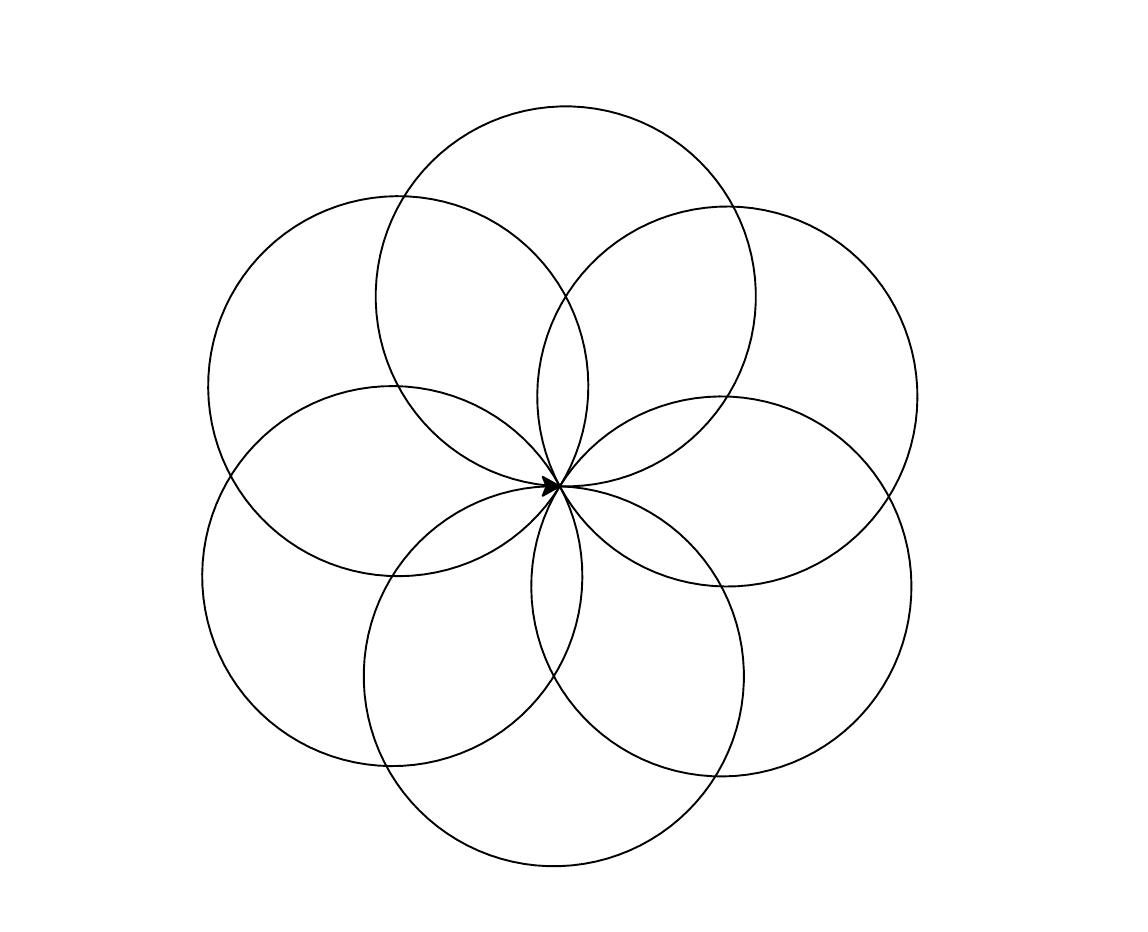
\includegraphics[scale=0.2]{imagenes/circulos}
 \end{center}

 \item Escribe otro programa que produzca esta otra figura:
 
 
 \begin{center}
  
\includegraphics[scale=0.2]{imagenes/flor}
 \end{center}

 
 
 
 \item Escribe un programa que produzca una casa como las que dibujan los
ni\~nos peque\~nos, hecha de segmentos y arcos de circunferencia. Intenta
producir el mayor n\'umero posible de los detalles que suelen incluir esas casas
(el \'arbol, el camino que lleva a la puerta, ?`el humo de la chimenea?, etc.)
 
 
 
 
 \item {\sc ?`Continuar\'a?}
 
 %\begin{lstlisting}
 
%\end{lstlisting}
 
 \end{enumerate}
 
 
 
 


\end{appendices}
